\documentclass[../../labo_tp5_main.tex]{subfiles}

\begin{document}

%capítulo
\subsection{Ejercicio 2}

\subsection{Señal Cuadrada}

\subsubsection{Desarrollo de Fourier}
El desarrollo en serie de Fourier de una onda cuadrada x(t), de frecuencia $f_0$ y de amplitud $A$ (tensión pico) resulta ser: \par
\begin{center}
$x(t) = \sum\frac{4\cdot A}{n\pi}sen(2\pi nf_{0}t),\,n>0,\,impar$
\end{center}
Donde $X_n = \frac{4\cdot A}{n\pi}$ son los coeficientes de Fourier de la serie, que definen la amplitud de cada armónico.\par
De la fórmula anterior se deduce que la señal cuadrada tiene compontes en frecuencias bajas y altas. Además, observamos que los múltiplos pares de la frecuencia fundamental se anulan, es decir, no agregan potencia.\par

\subsubsection{Simulación de amplitud y potencia de armónicos}

En particular, la consigna indica que la señal de entrada deberá tener una amplitud de $250mV_{pp}$ y una frecuencia $f_0 = 1.7MHz$. Como el generador fue configurado en HiZ en el punto anterior y quedó configurado de esta manera cuando las mediciones fueron realizadas, se deberá tener en cuenta la transferencia del circuito formado entre la resistencia del generador de $50\ohm$  en serie con los $50\ohm$ del analizador de espectros, sobre el cual se realizarán las mediciones de potencia, por lo que debe tenerse en cuenta el divisor resistivo que hace que se pierda un 50\% de la amplitud de la señal al ser medida por el analizador. Esto implica que las simulaciones para los armónicos deberán hacer hacerse con una amplitud de $250mV_{pp}$.\par
Simulando con MATLAB 20 armónicos de dicha señal obtenemos el siguiente espectro: \par

%\begin{figure}[H]	
	%\centering
	%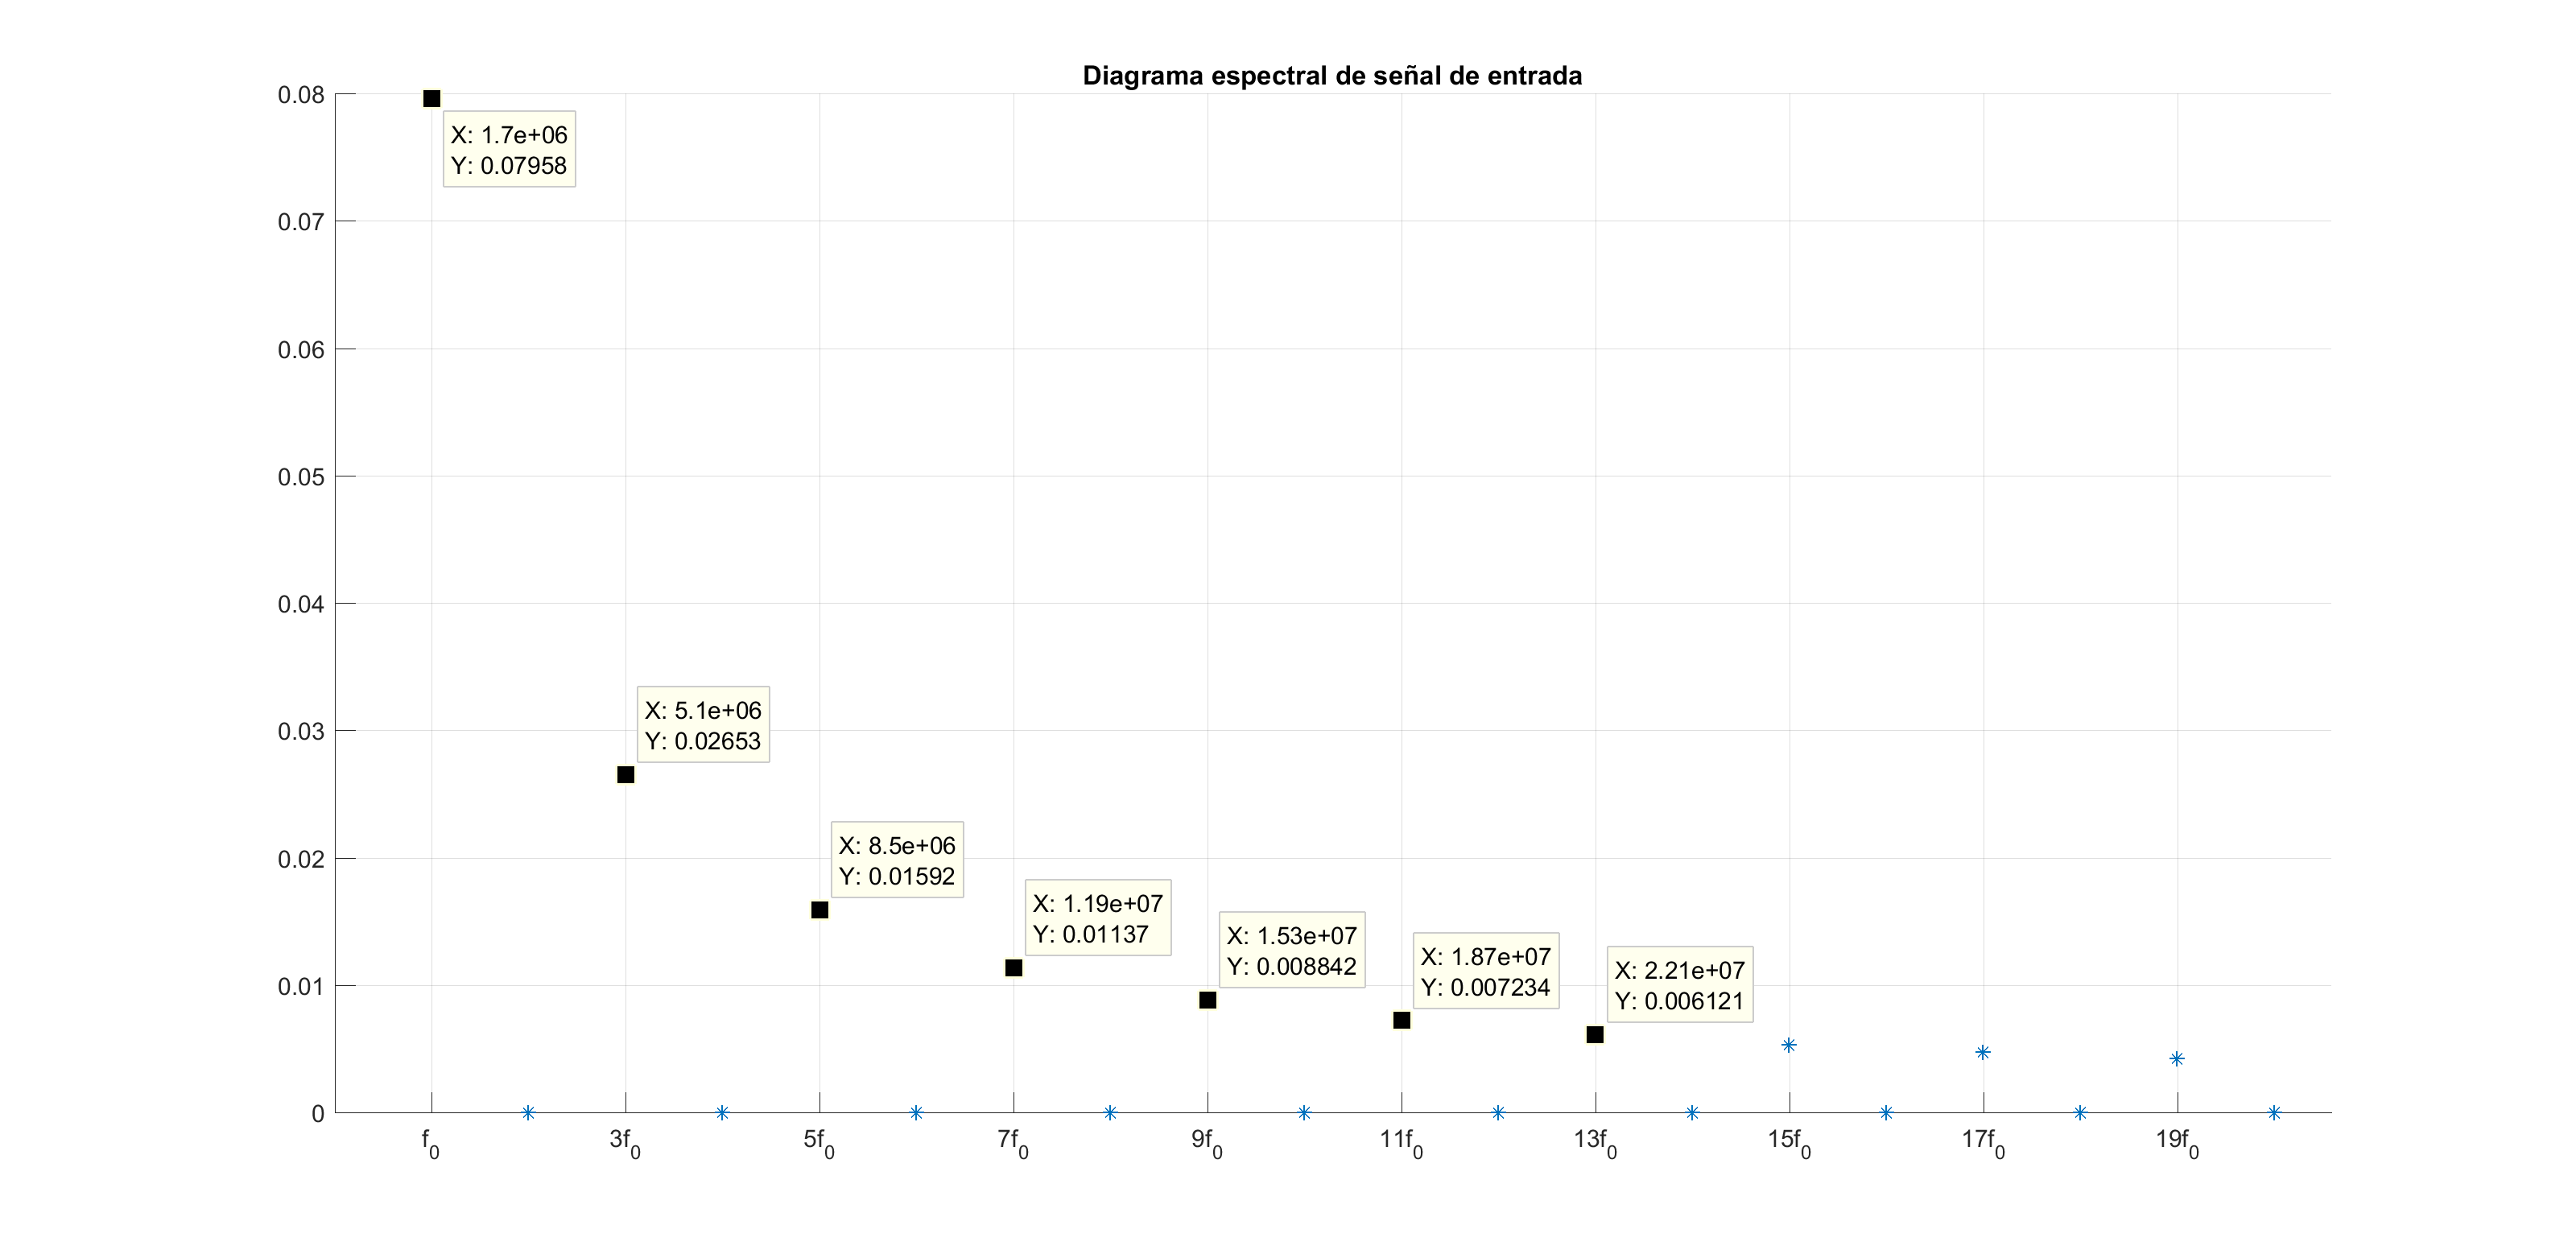
\includegraphics[scale=0.2]{imagenes/espectro_cuadrada_20_armonicos.png}
	%\caption{20 armónicos de la señal cuadrada de entrada}
	%\label{fig:ej1_espectro_cuadrada_20_armonicos}
%\end{figure}

Dada que la potencia estará ligada al cuadrado del módulo de la amplitud del armónico y teniendo en cuenta que esta potencia será medida sobre una resistencia de $50\ohm$, podemos simular también el diagrama espectral de potencia de la señal bajo la fórmula $\frac{|X_n|^2}{50}$:\par

%\begin{figure}[H]	
	%\centering
	%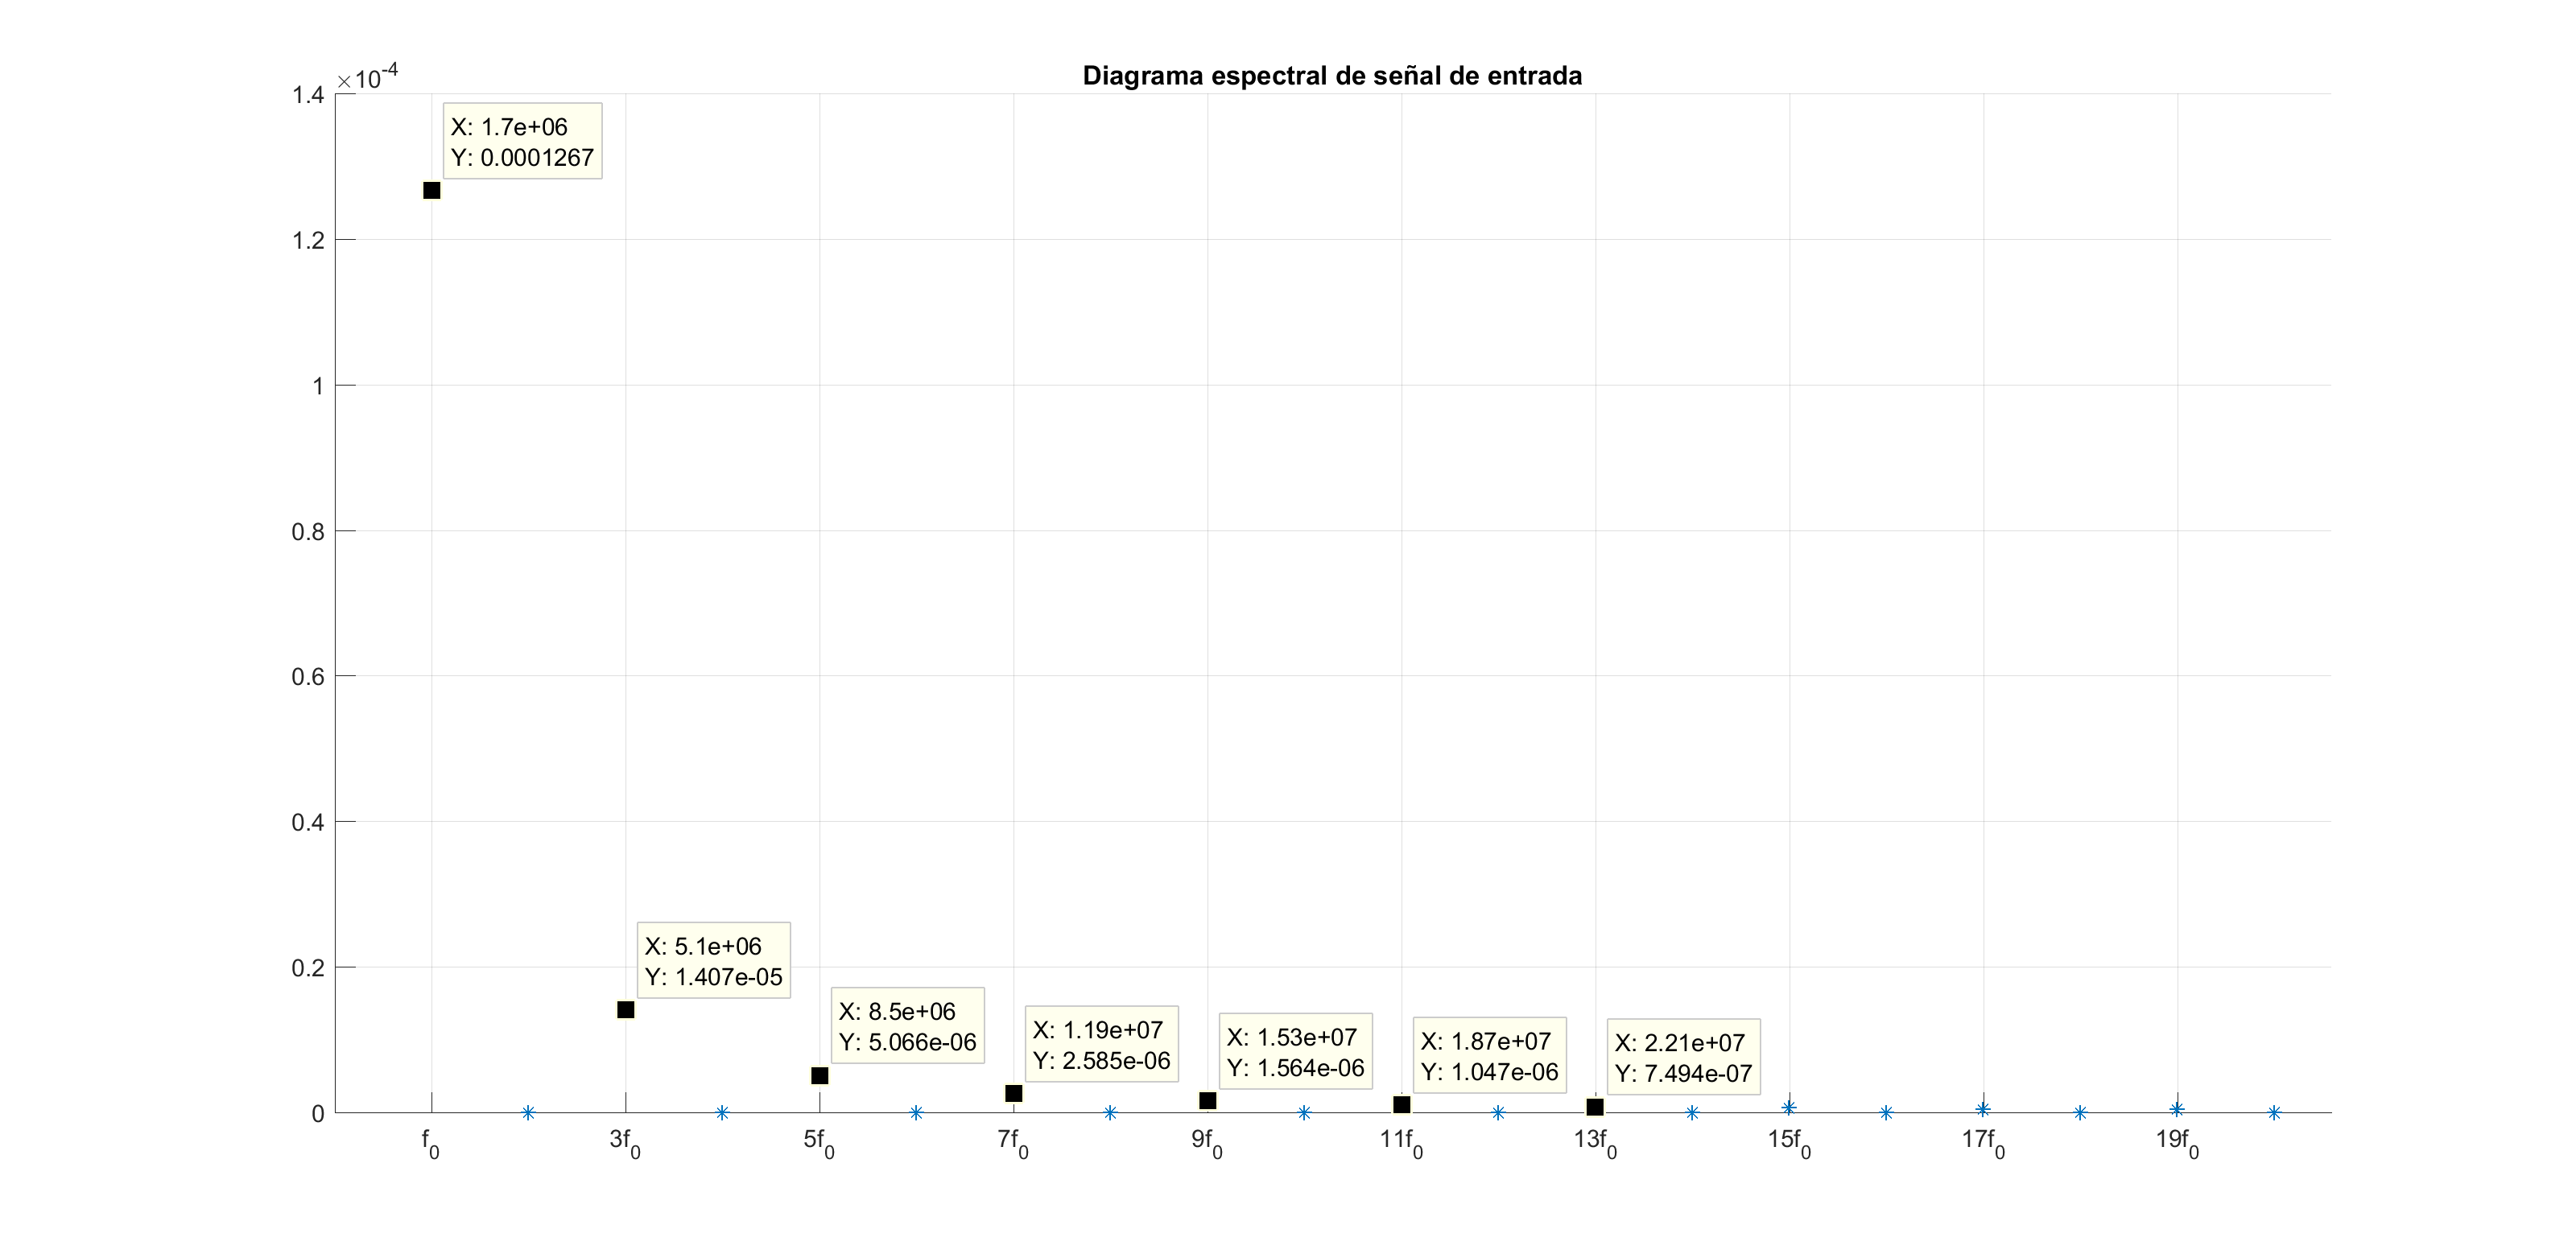
\includegraphics[scale=0.2]{imagenes/espectro_cuadrada_potencia.png}
	%\caption{20 armónicos de potencia para la señal cuadrada de entrada}
	%\label{fig:ej1_espectro_cuadrada_potencia}
%\end{figure}

Luego, utilizamos el analizador de espectros del laboratorio para poder medir la potencia de dichos armónicos. Para ello, fijamos la atenuación en 10dB y con el cursor seleccionamos el pico de cada armónico. De aquí obtuvimos la siguiente tabla de datos al haber medido como mínimo 10 armónicos para tener una medida representativa. Debe aclararse que como el generador no es ideal, la potencia de los armónicos pares no será nula, pero su potencia deberá ser indefectiblemente más pequeña que la de sus armónicos impares adyacentes.

\subsubsection{Mediciones y comparación de resultados}

\begin{table}[H] %señal cuadrada, mediciones
	\centering
 		\begin{tabular}{||c c c c||} 
 			\hline
			Armónico & Frecuencia (MHz) & Potencia (dBm) & Potencia (W)\\ [0.5ex] 
 			\hline\hline
			1 & $1.7MHz$ & -11.8 & $6.61\cdot 10^{-5}$\\
			2 & $3.4MHz$ & -62.4 & $5.75\cdot 10^{-10}$\\
			3 & $5.1MHz$ & -21 & $7.94\cdot 10^{-6}$\\
			4 & $6.8MHz$ & -71 & $7.94\cdot 10^{-11}$\\
			5 & $8.5MHz$ & -25.6 & $2.75\cdot 10^{-6}$\\
			6 & $10.2MHz$ & -70 & $1\cdot 10^{-10}$\\
			7 & $11.9MHz$ & -28.4 & $1.44\cdot 10^{-6}$\\
			8 & $13.6MHz$ & -72.4 & $5.75\cdot 10^{-11}$\\
			9 & $15.3MHz$ & -31.8 & $6.61\cdot 10^{-7}$\\
			10 & $17MHz$ & -77.4 & $1.81\cdot 10^{-11}$\\
			11 & $18.7MHz$ & -35.8 & $2.63\cdot 10^{-7}$\\[1ex] 
			\hline
		\end{tabular}
\end{table}
Hacemos notar de la tabla anterior que al multiplicar por un factor algo menor a dos a cada una de las potencias de los armónicos se obtienen los valores teóricos simulados con MATLAB. Se cree que este factor se debe al THD del generador, que es cercano al 50\% (medido en el ejercicio anterior), por lo que mitad de la potencia que se obtendría teóricamente se perdería en armónicos que no son de interés, en este caso los armónicos que teóricamente tendrían potencia nula. \par
El mismo fenómeno se observará por lo tanto para las distintas señales a generar y medir en el analizador, como lo serán la triangular y el tren de pulsos.\par

\subsubsection{Cálculo del Duty Cycle}

Planteando la señal cuadrada con duty cycle definido por el factor de escalamiento d, donde d<T, siendo T el período de la señal:\par
\begin{center}
$$x(t) = \sum_{k = -\infty}^{\infty}A\cdot\prod(\frac{t-k\cdot T}{d})$$
\end{center}
Se obtienen los coeficientes en serie trigonométrica de fourier para dicha señal:
	 \begin{equation}
  	   y(t) = \left\{
	  	    \begin{array}{ll}
		 					a_n = \frac{2\cdot A}{\pi\cdot n}\cdot sen(\frac{\pi\cdot n\cdot d}{T}) \\
			 				b_n = 0 \\
	     	 \end{array}
	     	\right.
 	\end{equation}
Por lo que el desarrollo en serie de fourier de x(t) queda expresado como:\par
\begin{center}
$$x(t) = \sum_{k = 1}^{\infty}\frac{2\cdot A}{\pi\cdot n}\cdot sen(\frac{\pi\cdot n\cdot d}{T})\cdot cos(\frac{2\pi\cdot n\cdot t}{T})$$
\end{center}
De esta manera, observando los armónicos que se anulan se podrá deducir la relación $\frac{d}{T}$ que determina el duty cycle.\par
Como en la serie anterior observamos que se anulan los armónicos pares, entonces $sen(\frac{\pi\cdot n\cdot d}{T}) = 0$, $\forall n = 2k$, con $k \epsilon \mathbb{Z}$. Por ende deducimos que $\frac{d}{T} = \frac{1}{2}$, por ende el duty cycle de la señal es del 50\%.

\subsection{Señal Triangular}
%http://mathworld.wolfram.com/FourierSeriesTriangleWave.html sacado de aca
\subsubsection{Desarrollo de Fourier}
El desarrollo en serie de Fourier de una onda triangular x(t), de frecuencia $f_0$ y de amplitud $A$ (tensión pico) resulta ser: \par
\begin{center}
$x(t) = \sum\frac{8\cdot A\cdot (-1)^\frac{n-1}{2}}{(n\cdot\pi)^2}\cdot sen(2\pi nf_{0}t),\,n>0,\,impar$
\end{center}
Donde $X_n = \frac{8\cdot A\cdot (-1)^\frac{n-1}{2}}{(n\cdot\pi)^2}$ son los coeficientes de Fourier de la serie, que definen la amplitud de cada armónico.\par

Se vuelve a observar que se anulan los armónicos pares por el duty cycle del 50\% y el hecho de que la señal triangular tiene simetría de media onda.\par
Dado que el generador no puede generar triangulares de mayor frecuencia , se seleccionó la frecuencia máxima como 200kHz.\par

\subsection{Simulación de potencia de armónicos}


\subsubsection{Mediciones y comparación de resultados}
\begin{table}[H] %señal triangular, mediciones
	\centering
 		\begin{tabular}{||c c c c||} 
 			\hline
			Armónico & Frecuencia (MHz) & Potencia (dBm) & Potencia (W)\\ [0.5ex] 
 			\hline\hline
			1 & $0.2MHz$ & -15.4 & $2.88\cdot 10^{-5}$\\
			2 & $0.4MHz$ & -56 & $2.51\cdot 10^{-9}$\\
			3 & $0.6MHz$ & -34.2 & $3.8\cdot 10^{-7}$\\
			4 & $0.8MHz$ & -69.8 & $1.05\cdot 10^{-10}$\\
			5 & $1MHz$ & -43 & $5.01\cdot 10^{-8}$\\[1ex] 
			\hline
		\end{tabular}
\end{table}


\subsection{Tren de pulsos}

Siguiendo la fórmula desarrollada en la sección sobre el cálculo del duty cycle, observamos que para la relación $d \cdot f_0= \frac{d}{T}= \frac{1}{3} $, (duty cycle del 33.33\%) se anularán los terceros armónicos de la señal\par

\subsubsection{Simulación de amplitud y potencia de armónicos}
El espectro simulado para el tren de pulsos es:\par
%
%\begin{figure}[H]	
	%\centering
	%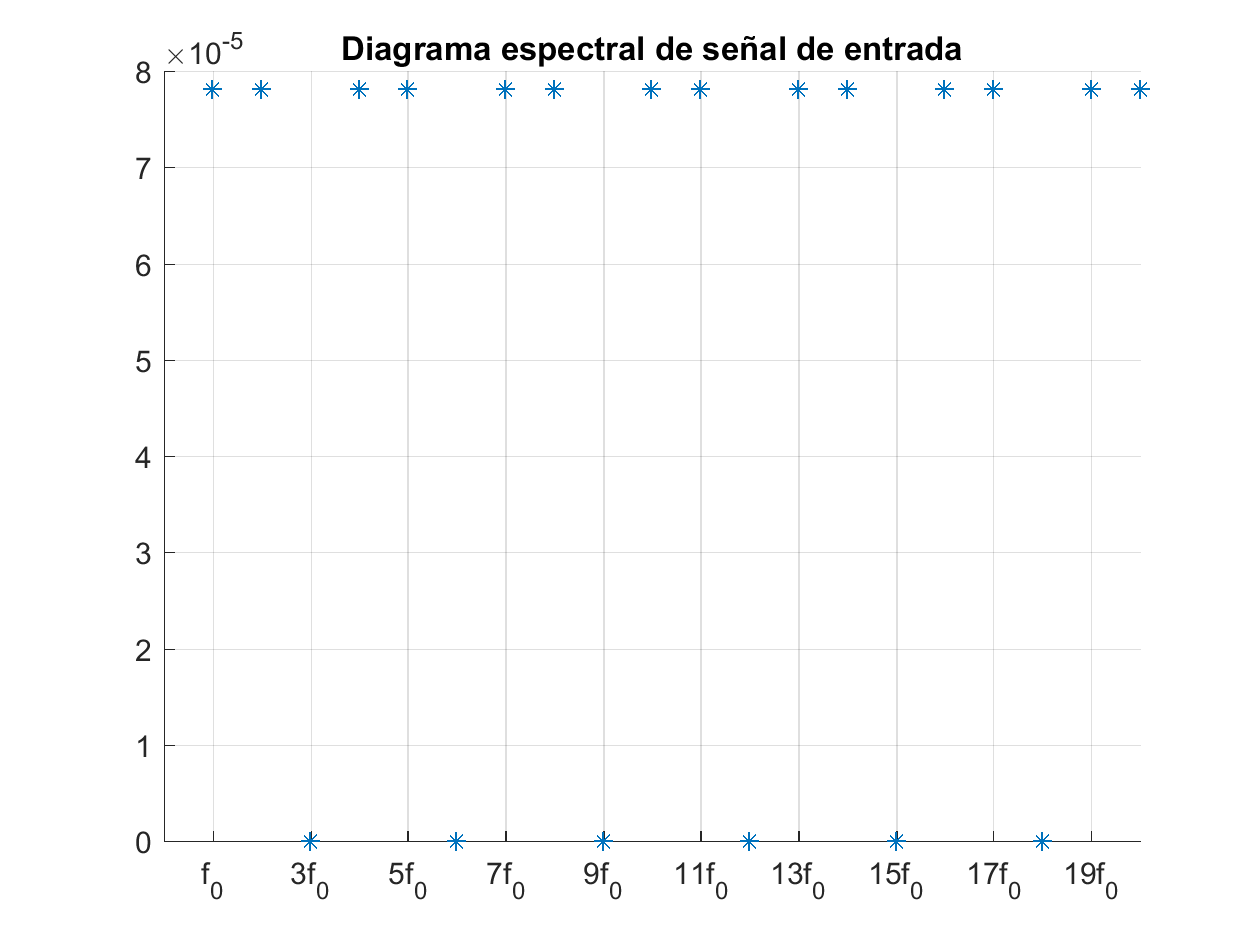
\includegraphics[scale=0.4]{imagenes/espectro_tren_pulsos.png}
	%\caption{20 armónicos de potencia para el tren de deltas}
	%\label{fig:ej1_espectro_tren_pulsos}
%\end{figure}

\subsubsection{Mediciones y comparación de resultados}
\begin{table}[H] %pulsos, mediciones
	\centering
 		\begin{tabular}{||c c c c||} 
 			\hline
			Armónico & Frecuencia (MHz) & Potencia (dBm) & Potencia (W)\\ [0.5ex] 
 			\hline\hline
			1 & $0.2MHz$ & -13.4 & $4.57\cdot 10^{-5}$\\
			2 & $0.4MHz$ & -19 & $1.25\cdot 10^{-5}$\\
			3 & $0.6MHz$ & -50.6 & $8.7\cdot 10^{-9}$\\
			4 & $0.8MHz$ & -25.2 & $3.02\cdot 10^{-6}$\\
			5 & $1MHz$ & -26.6 & $2.18\cdot 10^{-6}$\\
			6 & $1.2MHz$ & -50 & $1\cdot 10^{-8}$\\
			7 & $1.4MHz$ & -30.4 & $9.12\cdot 10^{-7}$\\
			8 & $1.6MHz$ & -30.8 & $8.32\cdot 10^{-7}$\\
			9 & $1.8MHz$ & -50.8 & $8.32\cdot 10^{-9}$\\
			10 & $2MHz$ & -33.8 & $4.16\cdot 10^{-7}$\\
			11 & $2.2MHz$ & -33.4 & $4.57\cdot 10^{-7}$\\[1ex] 
			\hline
		\end{tabular}
\end{table}

